% %%%%%%%%%%%%%%%%%%%%%%%%%%%%%%%%%%%%%%%%%%%%%%%%%%%%%%%%%%%%%%%%%%%%%%%%%%%%%
% %%%%%%%%%%%%%%%%%%%%%%%%%%%%%%%%%%%%%%%%%%%%%%%%%% Results of Numerical Model
% %%%%%%%%%%%%%%%%%%%%%%%%%%%%%%%%%%%%%%%%%%%%%%%%%%%%%%%%%%%%%%%%%%%%%%%%%%%%%

\chapter{Electron Inertial Effects}
\label{ch_inertia}

\todo{Note that Bob's 2011 paper\cite{lysak_2011} had inertial effects. }

\todo{Parallel electric fields and field-aligned currents are topics of particular interest. }

The model described in \cref{ch_model} has the notable omission of parallel electric fields and parallel currents. That situation can be remedied by the addition of the electron inertial term in \ohmlaw. 

Old parallel electric field formulation. Recall $\vec{F} \equiv \curl{B}$. 
\begin{align}
  \ez \ddt E_\parallel &= \frac{1}{\mu_0} F_\parallel - \sz E_\parallel
\end{align}

New parallel electric field formulation. The parallel current must now be tracked explicitly. 
\begin{align}
  \label{def_inertia}
  \ez \ddt E_\parallel &= \frac{1}{\mu_0} F_\parallel - J_\parallel &
  \ddt J_\parallel &= \frac{n e^2}{m} E_\parallel - \nu J_\parallel
\end{align}

In the new formulation, $J_\parallel$ (proportional to $J_3$) is solved with integrating factors and $E_\parallel$ ($E_3$) can be advanced directly. 
\begin{align}
  \begin{split}
  E_3 &\assign E_3 + c^2 \dt \, \lr{ g_{31} F^1 + g_{33} F^3 } - \frac{\dt}{\ez} J_3 \\
  J_3 &\assign J_3 \exp \arg{ - \nu \dt } + \frac{n e^2}{m} \dt \, E_3 \exp \arg{ -\nu \tfrac{\dt}{2} }
  \end{split}
\end{align}

Recall that the electric and magnetic fields are staggered by half a time step. The current is defined with the magnetic fields, offset from the electric fields. 

\todo{Note that \cref{ch_azm,ch_rbsp} don't use inertial effects. we just look at them here as a proof of concept. Resolving inertial length scales is too expensive, and not resolving them can easily lead to instability. }

% =============================================================================
% =============================================================================
% =============================================================================
\section{The Boris Approximation}
  \label{sec_boris}

Note that 
\begin{align}
  \ddt E_\parallel &\sim -\frac{1}{\ez} J_\parallel &
  & \text{and} & 
  \ddt J_\parallel &\sim \frac{n e^2}{\me} E_\parallel &
  & \text{so} &
  \frac{ \partial^2 }{ \partial t^2 } E_\parallel &\sim -\op^2 E_\parallel
\end{align}

That is, the addition of the electron inertial term in \ohmlaw allows plasma oscillations. 

As noted in \cref{sec_e}, the plasma frequency is very large. Much larger than $\frac{1}{\dt}$. But $\op \dt < 1$ is necessary for stability. In order to accommodate that condition, the time step in some runs would need to be dropped by three orders of magnitude; a simulation slated for one hour would suddenly take six weeks to complete. 

The time step dictated by the \Alfven speed and grid spacing is typically on the order of $\SI{10}{\us}$, while the plasma frequency can be as small as $\SI{10}{\ns}$. 

The plasma frequency (and the speed of light) can be decreased by taking an artificially large value for \ez. Such approximations have been staples of numerical MHD models since Boris' work in 1970\cite{boris_1970}.

Lysak and Song\cite{lysak_2001} demonstrate the validity of such an approximation. To paraphrase their work, take \cref{def_inertia} and suppose that $E_\parallel$ and $J_\parallel$ are oscillating at a frequency $\omega$. Then,
\begin{align}
  - i \omega \ez E_\parallel &= \oomz F_\parallel - J_\parallel & - i \omega J_\parallel &= \frac{n e^2}{\me} E_\parallel - \nu J_\parallel
\end{align}

So
\begin{align}
  \label{boris_criterion}
  \lr{ 1 - \frac{\omega^2 - i \nu \omega}{\op^2} } E_\parallel &= \frac{c^2}{\op^2} \lr{ \nu - i \omega } F_\parallel
\end{align}

Here $\frac{c}{\op}$ is the electron inertial length. While the speed of light and the plasma frequency each depend on \ez, their ratio does not. So long as $\lr{ 1 - \frac{\omega^2 - i \nu \omega}{\op^2} } \sim 1$, a change in \ez should not affect model behavior. 

For the purposes of simulating ultra low frequency waves, \cref{boris_criterion} allows perhaps-implausibly large Boris factors; even increasing \ez by a factor of \num{e6} gives $\left| \frac{\omega^2 + i \omega \nu}{ \op^2 } \right| \lesssim 0.01$. At that point, in some places, the speed of light is significantly slower than the \Alfven speed. 

\todo{Ronnmark\cite{ronnmark_2000} calls this ``anisotropic vacuum.'' }

\todo{This is common in other models... very high ionosphere, low speed of light, whatever. Cite LFM or something? }

\todo{Plot of these frequency ratios in the ionosphere? }

\todo{Generalized \ohmlaw, in case we decide we need it. Could talk through why all of the other terms are OK to neglect.  
\begin{align}
  \vec{E} + \cross{U}{B} & = 
  \eta \vec{J} + \tfrac{\me}{n e^2} \lrb{
    \tfrac{\partial}{\partial t} \vec{J} + \nabla \cdot \lr{ 
      \vec{J} \, \vec{U} + \vec{U} \,\vec{J} +
      \tfrac{1}{n e} \vec{J} \, \vec{J} } } +
  \tfrac{1}{n e} \cross{J}{B} -
  \tfrac{1}{n e} \div{ \vec{P_e} }
\end{align}
}

% =============================================================================
% =============================================================================
% =============================================================================
\section{Effect on the Simulation}

\begin{figure}[H]
    \centering
    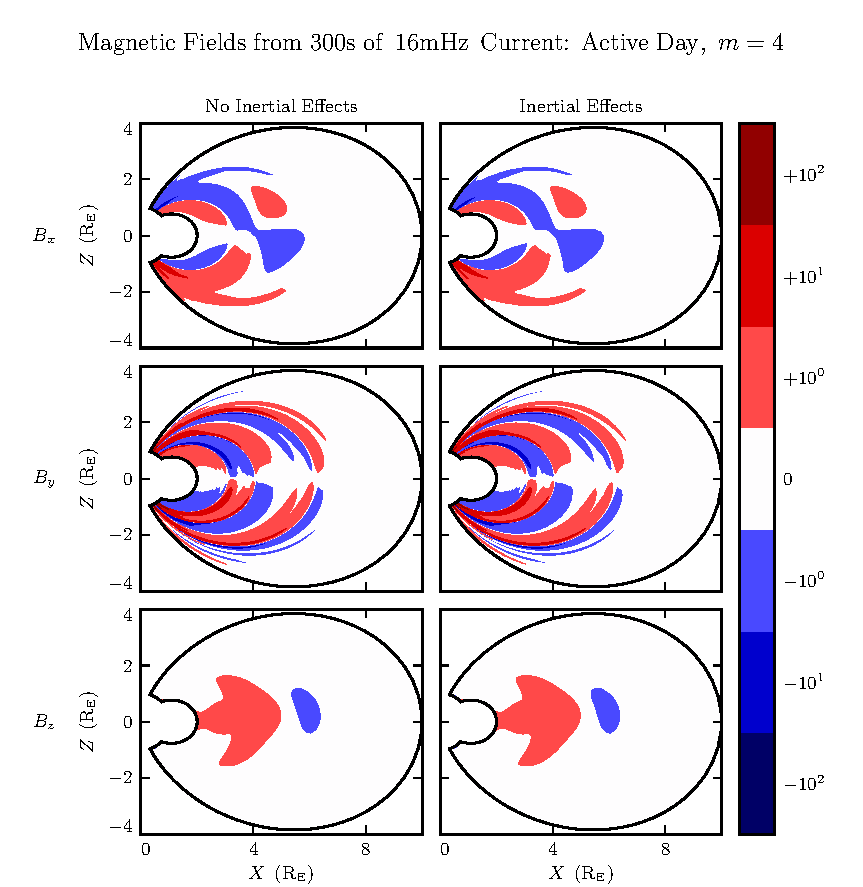
\includegraphics[width=\textwidth]{figures/B_1_004_016mHz.pdf}
    \caption[Magnetic Field Comparison With and Without Electron Inertial Effects]{
      The addition of electron inertial effects, with no other changes to the model, does not visible change the output. In a way, this is reassuring, since the alternative is to cast doubt on past work. 
    }
    \label{fig_B_1_004_016mHz}
\end{figure}

% =============================================================================
% =============================================================================
% =============================================================================
\section{Field-Aligned Current}
  \label{sec_fac}

Over the bulk of the simulation, each field is overwhelmingly real or imaginary. Driving is injected into the real poloidal electric field, giving real $E_x$ and $B_y$ (and real $B_z$, at least for low \azm... at large \azm, the compressional magnetic field becomes very small). Toroidal components -- $E_x$ and $B_y$ -- are imaginary, indicating an azimuthal offset. 

This comes from the curls in \farlaw and \amplaw; a derivative in the azimuthal direction comes with a factor of $i$. 

By that reasoning, it seems that the parallel electric field $E_z$ should line up with the toroidal mode. 

The distinction between real and imaginary fields gets muddled at the ionosphere, since (imaginary) $E_x$ and (real) $E_y$ are coupled by the Hall conductivity. 

The finer points are still being worked out. 

\begin{figure}[H]
    \centering
    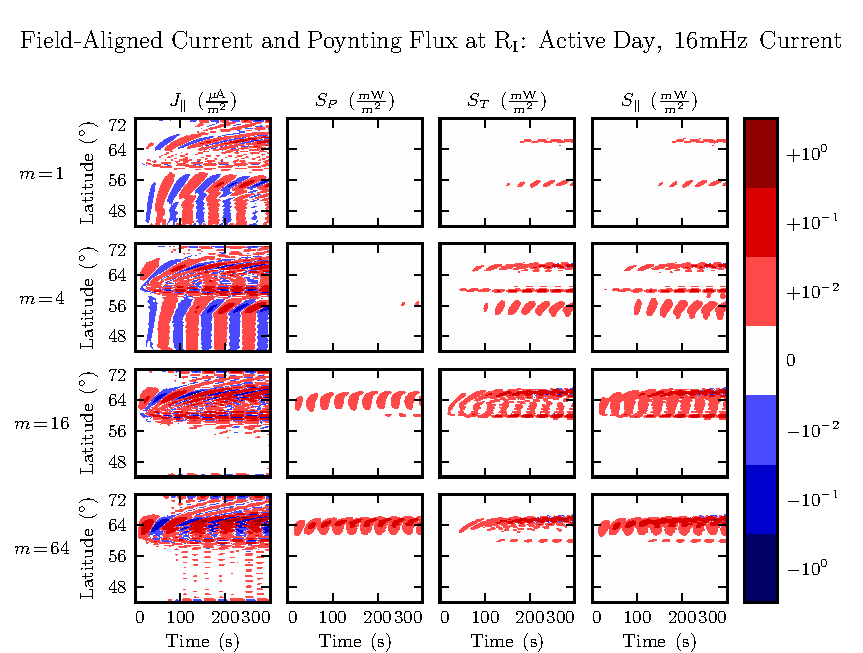
\includegraphics[width=\textwidth]{figures/JS_1_016mHz.pdf}
    \caption[Field-Aligned Current and Poynting Flux at the Ionosphere]{
      Perhaps unsurprisingly, field-aligned current structures at the ionospheric bounadry line up with Poynting flux structures. The imaginary component of the current lines up with the (imaginary) toroidal Poynting flux, while the real current lines up with the poloidal Poynting flux. 
    }
    \label{fig_JS_1_016mHz}
\end{figure}

\todo{Notably, while the net Poynting flux is downward almost everywhere, field-aligned currents alternate between upward and downward flow. Perhaps this has to do with Poynting flux being a quadratic quantity while current is linear? Check the phases of the electric and magnetic fields. }

The ``wigglies'' visible in the lower-left corner of \cref{fig_JS_1_016mHz} suggests overcorrection due to an improperly-coarse grid. See \cref{sec_lengths}. 


\begin{figure}[H]
    \centering
    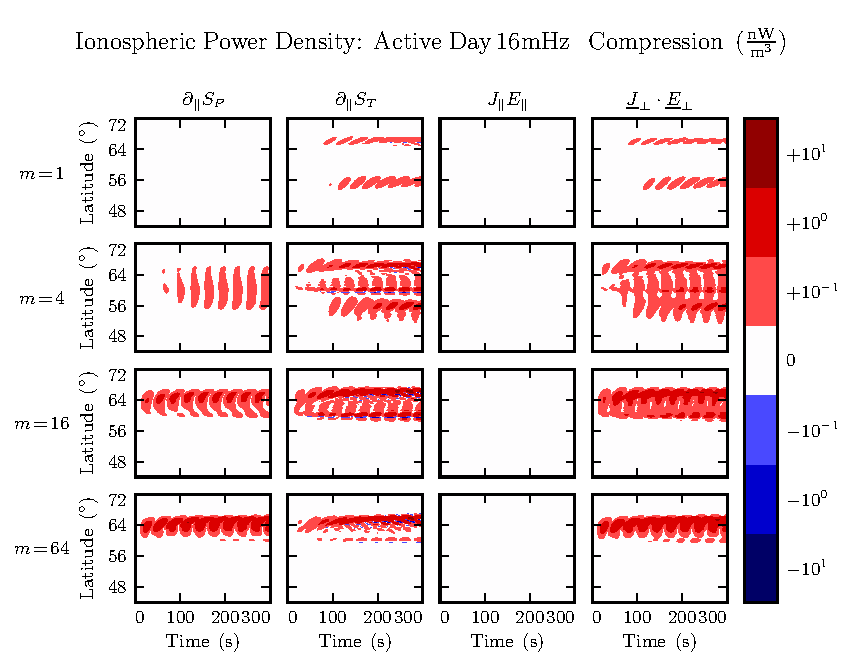
\includegraphics[width=\textwidth]{figures/JE_1_016mHz.pdf}
    \caption[Ionospheric Power Density]{
      While field-aligned currents can be of significant size, they are not particularly good at depositing energy in the ionosphere. Energy deposited by the Poynting flux matches closely with Joule dissipation from the perpendicular currents -- energy conservation! -- while $J_\parallel E_\parallel$ is smaller by several orders of magnitude. 
    }
    \label{fig_JE_1_016mHz}
\end{figure}

% =============================================================================
% =============================================================================
% =============================================================================
\section{Inertial Length Scales}
  \label{sec_lengths}

A typical run has maximum $E_y$ on the order of \SI{10}{\mV/\meter} and maximum $E_z$ on the order of \SI{e-3}{\mV/\meter}. Notably, however, it's the electric field derivative that affects the magnetic field, not its magnitude. 

At the ionospheric boundary, signatures in $E_y$ can vary on length scales of about \SI{1}{\degree}. This gives $\dd{x} E_y \dt \sim \SI{e-3}{nT/\second}$. 

The usual grid can't resolve features much smaller than that. But, recall from \cref{sec_boris}, that simulations now include plasma oscillation, for which the characteristic length scale is the electron inertial length, $\frac{c}{\op}$. 

The electron inertial length bottoms out below $\SI{e-1}{\km}$ inside the plasmasphere, and $\SI{1}{\km}$ outside it. 

The very small $E_z$ values being seen are unlikely to dominate $E_x$, but if inertial length scales were resolved in the perpendicular direction then $\dd{x} E_z \dt$ could be as large as \SI{e-4}{nT/\second}. 

Resolving electron inertial lengths is computationally very expensive. 

The range of $L$ values is decreased from \SIrange{2}{10}{\RE} down to \SIrange{5}{7}{\RE}. The number of grid points in the perpendicular direction is increased by a factor of five. This drops the time step by an order of magnitude -- smaller zones have smaller crossing times! 

All in all, a run that resolves inertial length scales is a factor of 100 more expensive than one that doesn't. 

\todo{Several such runs are going right now. They should finish over the weekend. Then we can see what our tiny grid spacing buys us! }





